%allgemeine Formatangaben
\documentclass[
 a4paper, 										% Papierformat
 12pt,												% Schriftgröße
 ngerman, 										% für Umlaute, Silbentrennung etc.
 titlepage,										% es wird eine Titelseite verwendet
 oneside, 										% einseitiges Dokument
 captions=nooneline,					% einzeilige Gleitobjekttitel ohne Sonderbehandlung wie mehrzeilige Gleitobjekttitel behandeln
 numbers=noenddot,						% Überschriften-??Nummerierung ohne Punkt am Ende
 parskip=half,									% zwischen Absätzen wird eine halbe Zeile eingefügt
 ]{scrartcl}

% Anpassung an Landessprache
\usepackage[ngerman]{babel}	

\usepackage[T1]{fontenc}	
\usepackage[utf8]{inputenc}	
\usepackage{textcomp} 																% Euro-Zeichen und andere
\usepackage[babel,german=quotes]{csquotes}						% Anführungszeichen
\RequirePackage[ngerman=ngerman-x-latest]{hyphsubst} 	% erweiterte Silbentrennung

% Befehle aus AMSTeX für mathematische Symbole z.B. \boldsymbol \mathbb
\usepackage{amsmath,amsfonts}

% Zeilenabstände und Seitenränder 
\usepackage{setspace}
\usepackage{geometry}

% Einbinden von JPG-Grafiken
\usepackage{graphicx}

% zum Umfließen von Bildern
% Verwendung unter http://de.wikibooks.org/wiki/LaTeX-Kompendium:_Baukastensystem#textumflossene_Bilder
\usepackage{floatflt}

% Verwendung von vordefinierten Farbnamen zur Colorierung
% Palette und Verwendung unter http://kitt.cl.uzh.ch/kitt/CLinZ.CH/src/Kurse/archiv/LaTeX-Kurs-Farben.pdf
\usepackage[usenames,dvipsnames]{color} 

% Tabellen
\usepackage{array}
\usepackage{longtable}

% einfache Grafiken im Code
% Einführung unter http://www.math.uni-rostock.de/~dittmer/bsp/pstricks-bsp.pdf
\usepackage{pstricks}

% Quellcodeansichten
\usepackage{verbatim}
\usepackage{moreverb} 											% für erweiterte Optionen der verbatim Umgebung
% Befehle und Beispiele unter http://www.ctex.org/documents/packages/verbatim/moreverb.pdf
\usepackage{listings} 											% für angepasste Quellcodeansichten siehe
% Kurzeinführung unter http://blog.robert-kummer.de/2006/04/latex-quellcode-listing.html

% verlinktes und Farblich angepasstes Inhaltsverzeichnis
\usepackage[pdftex,
colorlinks=true,
linkcolor=InterneLinkfarbe,
urlcolor=ExterneLinkfarbe]{hyperref}
\usepackage[all]{hypcap}

% URL verlinken, lange URLs umbrechen
\usepackage{url}

% sorgt dafür, dass Leerzeichen hinter parameterlosen Makros nicht als Makroendezeichen interpretiert werden
\usepackage{xspace}

% Beschriftungen für Abbildungen und Tabellen
\usepackage{caption}

% Entwicklerwarnmeldungen entfernen
\usepackage{scrhack}

\newcommand{\qq}[1]{\glqq{#1\grqq{}}} %Gänsefüßchen

\onehalfspacing 							% 1,5facher Zeilenabstand

\definecolor{InterneLinkfarbe}{rgb}{0.1,0.1,0.3} 	% Farbliche Absetzung von externen Links
\definecolor{ExterneLinkfarbe}{rgb}{0.1,0.1,0.7}	% Farbliche Absetzung von internen Links

% Einstellungen für Fußnoten:
\captionsetup{font=footnotesize,labelfont=sc,singlelinecheck=true,margin={5mm,5mm}}					
\title{Abschlussbericht für das Modul SmartCard-Programmeriung}
\subtitle{Implementierung einer MultiCard-Anwendung\vspace{1cm}}

\author{B. Sc. Andrej Lisnitzki, B. Sc. Michael Horn}
\date{\today}
\begin{document}
\maketitle

\tableofcontents
\pagebreak

\section{Einleitung}
In dem Projekt \qq{Implementierung einer MultiCard} für das Wahlpflichtmodul \qq{SmartCard-Programmierung} im Sommersemester 2016 geht es um eine beispielhafte Realisierung einer SmartCard-Anwendung.
Zu einer SmartCard-Anwendung gehören sogenannte On- und OffCard-Teile.
Der OnCard-Teil beschreibt die Anwendung auf der SmartCard, während der OffCard-Teil die Nutzerseite beschreibt.

In dem Projekt \qq{Implementierung einer MultiCard} sollen mögliche Anwendungen für eine Studenten- und Discokarte realisiert werden.
Gleichermaßen soll jegliche Kommunikation kryptographisch verschlüsselt erfolgen, damit eine Manipulation der Karte beziehungsweise der Daten auf der Karte verhindert werden.

\paragraph{Aufgabe:}
Es sollte eine SmartCard-Anwendung entstehen, welche als Bestandteile zum Einen eine Studenten-Karte realisiert.
Zum Anderen soll die SmartCard eine sogenannte Disco-Karte realisieren.
Weiterhin soll die komplette Kommunikation verschlüsselt erfolgen.

Bestandteile der Student-Anwendung sind:
\begin{itemize}
	\item Studentenname und Matrikel
	\item Raumzugänge
	\item Geld einzahlen und per Essen verbrauchen
	\item Daten abfragen
\end{itemize}

Bestandteile der Disco-Anwendung sind:
\begin{itemize}
	\item Geld einzahlen
	\item Konsumierte Getränke speichern und bezahlen
	\item Bonuspunkte für Konsum und verbrauchen der Punkte
	\item Daten abfragen
\end{itemize}

Bestandteile der Kryptographie sind:
\begin{itemize}
	\item Verschlüsseln
	\item Entschlüsseln
	\item Signierung
\end{itemize}

\paragraph{Verlauf:}
Im Verlauf des Projektes wurden die Anforderungen entsprechend der Aufgabe realisiert.
Das gesamte Projekt wurde per sogenanntem \qq{Pair-Programming} realisiert.
\qq{Pair-Programming} bezeichnet das gemeinsame Programmieren an einem Bildschirm, während einer das Programm schreibt denkt der jeweils andere über das geschriebene nach.
Regelmäßig werden diese beiden Rollen getauscht.

\paragraph{Ergebnis:}
Als Ergebnis des Projektes entstand eine kryptographisch gesicherte SmartCard-Anwendung, welche ein Studenten-, Disco- und Crypto-Applet enthält.
Außerdem entstand eine OffCard-Anwendung welche diese Funktionalitäten der SmartCard anspricht.
Der einfachheitshalber wurde die OffCard-Anwendung in Tabs untergliedern um die verschiedenen Einsatzbereiche abzutrennen.

\paragraph{Aufbau:}
In diesem Bericht wird zunächst auf die verschiedenen Applets mit Ihren Anweisungen und den verschiedenen Fehlern eingegangen.
Im Anschluss an den OnCard-Teil wird auf den OffCard-Teil eingegangen.
Am Ende des Berichtes wird ein Fazit über das realisierte Projekte gezogen.

\subsection{Simulation}
\label{label:simulation}
Das komplette Projekt wurde unter Linux entwickelt.
Unter den verwendeten Systemen Linux Mint 17.3 und Ubuntu 15.10 existieren keine Treiber für JavaCard-Lesegeräte.
Dadurch wurde das gesamte Projekt mit Hilfe der Simulation per JCOP getestet.

Damit die OffCard-Anwendung mit der simulierten SmartCard und damit mit dem OnCard-Teil kommunizieren kann, muss die opencard.properties für die Simulation konfiguriert sein.
Im Anschluss muss die Simulation per JCOP in Eclipse gestartet werden.
Wichtig ist das die AIDs in Eclipse richtig gesetzt sind, siehe dazu \autoref{label:oncard} und alle Applets müssen korrekt installiert sein.
Außerdem wichtig ist, dass zur Simulation der Port 8050 verwendet wird und geöffnet ist.
In der JCOP-Shell muss in Eclipse im Anschluss explizit ein /close ausgeführt werden, damit die Verbindung freigegeben wird.
Erst dann kann sich die OffCard-Anwendung mit SmartCard korrekt verbinden und die Anwendung verwendet werden.

\section{Oncard}
\label{label:oncard}

Die Package-AID des multiCard-Packages ist multiCard in hexadezimal geschrieben:
\begin{itemize}
	\item 0x 6d 75 6c 74 69 43 61 72 64
\end{itemize}

Innerhalb der Applets auf der SmartCard wurden zum Teil eigene Fehler definiert.
Dies erleichtert die Lokalisierung von Fehlern und Problemen bei der Abarbeitung von Anweisungen auf der SmartCard.
Falls ein Fehler auftritt, wird dieser an die OffCard-Anwendung weitergeleitet und entsprechend behandelt.
Die selbst definierten Fehler-Codes werden nachfolgend bei den entsprechenden Applets angegeben.

Zu den selbst definierten Fehler-Codes können noch folgende allgemeine Fehler auftreten:
\begin{itemize}
	\item ISO7816.SW\_CLA\_NOT\_SUPPORTED
	\begin{itemize}
		\item Klassenbyte wird nicht unterstützt.
	\end{itemize}
	\item ISO7816.SW\_INS\_NOT\_SUPPORTED
	\begin{itemize}
		\item Anweisung wird nicht unterstützt.
	\end{itemize}
	\item ISO7816.SW\_WRONG\_LENGTH
	\begin{itemize}
		\item Daten haben falsche Länge.
	\end{itemize}
	\item ISO7816.SW\_DATA\_INVALID)
	\begin{itemize}
		\item Daten sind ungültig (wurden manipuliert).
	\end{itemize}
\end{itemize}

Der OnCard-Teil enthält die drei Applets: Student, Disco und Crypto.

\subsection{Student-Applet}

Die AID des Student-Applets ist Student in hexadezimal geschrieben:
\begin{itemize}
	\item 0x 53 74 75 64 65 6e 74
\end{itemize}
Das Klassenbyte für das Student-Applet ist:
\begin{itemize}
	\item 0x 20
\end{itemize}

Das Student-Applet unterteilt sich in drei Komponenten.
Zum Einen die Funktionalität mit Geld umzugehen und zum Anderen das Speichern von Studentennamen sowie die Raumfreischaltungen.
Das Essen in der Mensa auf der Studentenkarte wird durch einfaches Geld ausgeben realisiert.

\subsubsection{Geld}
\label{label:geld}
Im Student-Applet kann Geld eingezahlt und verbraucht werden, dabei wird Euro und Cent jeweils als 1 Byte dargestellt.
Auf der Karte wird zwischen ganzzahligem Euro-Betrag und Cent-Betrag unterschieden.
Daraus ergibt sich für den Euro-Betrag eine Obergrenze von 127\texteuro{}, da sonst ein Überlauf des Bytes erfolgen würde.
Die Höchstgrenze für den Cent-Betrag ist auf 99\textcent{} gesetzt.
Sodass der Höchstbetrag auf der Karte 127,99\texteuro{} ist.

\paragraph{INS\_GET\_MONEY (0x20)}
Liefert das aktuell auf der Karte gespeicherte Guthaben.
\paragraph{INS\_ADD\_MONEY (0x21)}
Fügt der Karte Geld hinzu.

Folgende Fehler können geworfen werden:
\begin{itemize}
	\item ERROR\_ADD\_EURO\_OVERFLOW (0xE021)
	\begin{itemize}
		\item Es kann kein ganzzahliger Betrag mehr hinzugefügt werden, da sonst ein Überlauf entstehen würde.
	\end{itemize}
	\item ERROR\_ADD\_CENT\_OVERFLOW (0xE121)
	\begin{itemize}
		\item Bei dem hinzufügen von Cents, entsteht ein Überlauf im Euro. 
	\end{itemize}
	\item ERROR\_ADD\_MONEY\_OVERFLOW (0xE221)
	\begin{itemize}
		\item Hinzufügen von Euro und Cent sorgt für einen Überlauf.
	\end{itemize}
\end{itemize}

\paragraph{INS\_SUB\_MONEY (0x22)}
Es wird ein Betrag vom Geld subtrahiert und damit ausgegeben.

Folgende Fehler können geworfen werden:
 \begin{itemize}
 	\item ERROR\_SUB\_EURO\_UNDERFLOW (0xE022)
 	\begin{itemize}
 		\item Subtraktion von Euro führt zu einem Unterlauf des Guthabens.
 	\end{itemize}
 	 \item ERROR\_SUB\_CENT\_UNDERFLOW (0xE122)
 	\begin{itemize}
 		\item Subtraktion von Cents führt zu einem Unterlauf des Guthabens.
 	\end{itemize}
 	 \item ERROR\_SUB\_INSUFFICIENT\_MONEY (0xE222)
 	\begin{itemize}
 		\item Nicht genügend Guthaben auf der Karte.
 	\end{itemize}
 \end{itemize}
 
\paragraph{INS\_RESET\_MONEY (0x23)}
Setzt Euro- und Cent-Betrag auf der Karte auf Null (Werkszustand).

\subsubsection{Studentendaten}
Auf der Karte wird der Name sowie die Matrikelnummer des Studenten gespeichert.

\paragraph{INS\_SET\_NAME (0x24)}
Schreibt den Namen des Studenten auf die Karte.
Der Name des Studenten darf maximal 50 Zeichen lang sein.

\paragraph{INS\_GET\_NAME (0x25)}
Liefert den gepeicherten Namen.

\paragraph{INS\_SET\_MATRIKEL (0x26)}
Setzt die Matrikelnummer des Studenten als Zahl (2 Byte).
Die Matrikelnummer darf höchstens 32767.

Folgende Fehler können geworfen werden:
\begin{itemize}
	\item ERROR\_SET\_MATRIKEL\_NEGATIVE (0xE025)
	\begin{itemize}
		\item Matrikelnummer darf nicht negativ sein.
	\end{itemize}
	\item ERROR\_SET\_MATRIKEL\_OVERFLOW (0xE125)
	\begin{itemize}
		\item Matrikel ist größer als höchstmöglicher Wert, wodurch ein Überlauf entstehen kann.
	\end{itemize}
\end{itemize}

\paragraph{INS\_GET\_MATRIKEL (0x27)}
Liefert die gespeicherte Matrikelnummer des Studenten.

\subsubsection{Raumfreischaltung}
Räume für den Studenten werden freigeschaltet in dem geprüft wird ob der Raum auf der SmartCard gespeichert ist (in Anlehnung an das System der HTWK Leipzig).
Damit Räume freigeschaltet werden können, werden diese als Liste auf der Karte gespeichert.
Es wird dabei immer die komplette Liste gesetzt beziehungsweise abgefragt.
Auf der Karte können maximal 16 Räume gespeichert werden.
Jeder Raum besteht aus drei Bytes.
Das erste Byte ist eine Enumeration für den Raumbuchstaben und die restlichen 2 Bytes dienen zur Darstellung der Raumnummer.

\paragraph{INS\_SET\_ROOMS (0x28)}
Speichert die als Liste übergebenen Räume auf der Karte.
\paragraph{INS\_GET\_ROOMS (0x29)}
Liefert eine Liste von gespeicherten Räumen auf der Karte

\subsection{Disco-Applet}
Die AID des Disco-Applets ist Disco in hexadezimal geschrieben:
\begin{itemize}
	\item 0x 44 69 73 63 6f
\end{itemize}
Das Klassenbyte für das Disco-Applet ist:
\begin{itemize}
	\item 0x 30
\end{itemize}

Das Disco-Applet besteht im Wesentlichen aus drei Komponenten.
Zum Einen das Sparen von Bonuspunkten durch Konsum von Getränken sowie das Speichern der verbrauchten Getränke auf der Karte.
Zum Anderen müssen die Getränke mit Hilfe von Geld (aus Student-Applet) und Bonuspunkten bezahlt werden. 
Geld-Funktionen im Disco-Applet kommunizieren durch die Applet-Firewall mit den Student-Applet (Sharable Object).
Üblicherweise wird die SmartCard bei Betreten der Lokalität vorgelegt und der Eintritt bezahlt.
Beim Verlassen der Lokalität wird die Karte wieder vorgelegt und entsprechender Getränkekonsum über die Karte bezahlt.

\subsubsection{Bonus}
Der Bonus wird als ein Byte gespeichert, daraus ergibt sich der maximale Bonus zu 127, da sonst ein Überlauf auftreten kann.
Bonuspunkte werden durch das konsumieren erhöht.
Die OffCard-Anwendung kümmert sich um die Verwaltung der Bonuspunkte.

\paragraph{INS\_GET\_BONUS (0x30)}
Liefert die aktuell gespeicherten Bonuspunkte.
\paragraph{INS\_ADD\_BONUS (0x31)}
Fügt Bonuspunkte hinzu.

Folgende Fehler können geworfen werden:
\begin{itemize}
	\item ERROR\_ADD\_BONUS\_OVERFLOW (0xE030)
	\begin{itemize}
		\item Es kann kein Bonus mehr hinzugefügt, da sonst ein Überlauf auftreten würde.
	\end{itemize}
\end{itemize}
\paragraph{INS\_SUB\_BONUS (0x32)}
Verbraucht Bonuspunkte.

Folgende Fehler können geworfen werden:
\begin{itemize}
	\item ERROR\_SUB\_BONUS\_UNDERFLOW (0xE031)
	\begin{itemize}
		\item Subtrahieren von Bonus würde ein Unterlauf-Fehler verursachen.
	\end{itemize}
	\item ERROR\_SUB\_INSUFFICIENT\_BONUS (0xE032)
	\begin{itemize}
		\item Nicht genug Bonuspunkte auf der Karte.
	\end{itemize}
\end{itemize}
\paragraph{INS\_RESET\_BONUS (0x33)}
Setzt die Bonuspunkte auf der Karte auf Null (Werkszustand).

\subsubsection{Geld}
Auf dem Disco-Applet können Geldfunktionen aus dem Student-Applet genutzt werden.
Dies ist nötig damit Student und Disco nicht über getrennte Guthaben verfügen müssen.
Kommunikation und der Zugriff auf das Geld des Student-Applet erfolgt über die Applet-Firewall (Sharable Object).
Die Anweisungen sind identisch zu den Anweisungen auf dem Student-Applet.
Für Details zu den Anweisungen wird auf \autoref{label:geld} verwiesen.

\subsubsection{Getränke}
Auf der SmartCard können maximal 50 Getränke gespeichert werden, welche in der Disco konsumiert wurden.
Für ein Getränk wird nur die ID als Byte in einer Liste gespeichert.
Der Preis zu dem Getränk wird durch die OffCard-Anwendung der ID zugeordnet.
	
\paragraph{INS\_GET\_DRINKS (0x34)}
Liefert eine Liste von konsumierten Getränken.
\paragraph{INS\_ADD\_DRINK (0x35)}
Fügt ein Getränk der Liste hinzu.

Folgender Fehler kann geworfen werden:
\begin{itemize}
	\item ERROR\_ADD\_DRINK\_HAD\_TO\_MUCH (0xE033)
	\begin{itemize}
		\item Getränkeliste ist voll, es können keine weiteren Getränke hinzugefügt werden.
	\end{itemize}
\end{itemize}

\paragraph{INS\_SET\_PAID\_DRINKS (0x36)}
Anhand einer übergebenen Liste, welche Einsen oder Nullen enthält, wird die interne Getränkeliste bereinigt, um Getränke welche bezahlt wurden.
Eine Eins entspricht dabei bereits bezahlt und eine Null noch zu bezahlen.
Die Übergebene Liste muss die gleiche Länge haben wie die derzeit gespeicherte Liste auf der Karte.

\subsection{Crypto-Applet}
Die AID des Crypto-Applets ist Crypto in hexadezimal geschrieben:
\begin{itemize}
	\item 0x 43 72 79 70 74 6f
\end{itemize}
Das Klassenbyte für das Crypto-Applet ist:
\begin{itemize}
	\item 0x 10
\end{itemize}

Das Crypto-Applet wurde geschaffen um Funktionen zu Verschlüsselung und Signierung für alle Applets über die Applet-Firewall zu bieten.
Im Crypto-Applet wird das asymmetrisches kryptographisches Verfahren RSA mit einer Schlüssellänge von 512 Bit realisiert.
Dieses Applet besitzt im Wesentlichen Funktionen zur Verschlüsselung und Signierung sowie zur Entschlüsselung und Verifizierung.

\subsubsection{Funktionsweise}
Das Crypto-Applet besitzt folgende Anweisungen:
\paragraph{INS\_IMPORT\_CARD\_PRIVATE\_MOD (0x10)} Importiert privaten Modulus des Schlüssel der Karte.

Folgender Fehler kann geworfen werden:
\begin{itemize}
	\item ERROR\_IMPORT\_CARD\_PRIVATE\_MOD (0xE010)
	\begin{itemize}
		\item Privater Modulus der Karte ist bereits auf der Karte gesetzt.
	\end{itemize}
\end{itemize}
\paragraph{INS\_IMPORT\_CARD\_PRIVATE\_EXP (0x11)} Importiert privaten Exponenten des Schlüssel der Karte.

Folgender Fehler kann geworfen werden:
\begin{itemize}
	\item ERROR\_IMPORT\_CARD\_PRIVATE\_EXP (0xE011)
	\begin{itemize}
		\item Privater Exponent der Karte ist bereits auf der Karte gesetzt.
	\end{itemize}
\end{itemize}
\paragraph{INS\_IMPORT\_CARD\_PUBLIC\_MOD (0x12)} Importiert öffentlichen Modulus des Schlüssel der Karte.

Folgender Fehler kann geworfen werden:
\begin{itemize}
	\item ERROR\_IMPORT\_CARD\_PUBLIC\_MOD (0xE012)
	\begin{itemize}
		\item Öffentlicher Modulus der Karte ist bereits auf der Karte gesetzt.
	\end{itemize}
\end{itemize}
\paragraph{INS\_IMPORT\_CARD\_PUBLIC\_EXP (0x13)} Importiert öffentlichen Exponenten des Schlüssel der Karte.

Folgender Fehler kann geworfen werden:
\begin{itemize}
	\item ERROR\_IMPORT\_CARD\_PUBLIC\_EXP (0xE013)
	\begin{itemize}
		\item Öffentlicher Exponent der Karte ist bereits auf der Karte gesetzt.
	\end{itemize}
\end{itemize}
\paragraph{INS\_EXPORT\_CARD\_PUBLIC\_MOD (0x14)} Exportiert öffentlichen Modulus des Schlüssel der Karte.

Folgender Fehler kann geworfen werden:
\begin{itemize}
	\item ERROR\_EXPORT\_CARD\_PUBLIC\_MOD (0xE014)
	\begin{itemize}
		\item Exportieren des öffentlichen Modulus des Schlüssel der Karte fehlgeschlagen.
	\end{itemize}
\end{itemize}
\paragraph{INS\_EXPORT\_CARD\_PUBLIC\_EXP (0x15)} Exportiert öffentlichen Exponenten des Schlüssel der Karte.

Folgender Fehler kann geworfen werden:
\begin{itemize}
	\item ERROR\_EXPORT\_CARD\_PUBLIC\_EXP (0xE015)
	\begin{itemize}
		\item Exportieren des öffentlichen Exponenten des Schlüssel der Karte fehlgeschlagen.
	\end{itemize}
\end{itemize}
\paragraph{INS\_IMPORT\_TERMINAL\_PUBLIC\_MOD (0x16)} Importiert öffentlichen Modulus des Schlüssel der OffCard-Anwendung.

Folgender Fehler kann geworfen werden:
\begin{itemize}
	\item ERROR\_IMPORT\_TERMINAL\_PUBLIC\_MOD (0xE016)
	\begin{itemize}
		\item Öffentlicher Modulus der OffCard-Anwendung ist bereits auf der Karte gesetzt.
	\end{itemize}
\end{itemize}
\paragraph{INS\_IMPORT\_TERMINAL\_PUBLIC\_EXP (0x17)} Importiert öffentlichen Exponenten des Schlüssel der OffCard-Anwendung.

Folgender Fehler kann geworfen werden:
\begin{itemize}
	\item ERROR\_IMPORT\_TERMINAL\_PUBLIC\_EXP (0xE017)
	\begin{itemize}
		\item Öffentlicher Exponenten der OffCard-Anwendung ist bereits auf der Karte gesetzt.
	\end{itemize}
\end{itemize}

Über die Instruktionen werden öffentliche und private Schlüssel auf die Karte importiert.
Die OffCard-Anwendung besitzt ein öffentliches und privates Schlüsselpaar.
Ebenfalls besitzt die SmartCard so ein Schlüsselpaar.
Wird das Applet installiert so sind keine Schlüssel gesetzt, so dass keine Verschlüsselung und Entschlüsselung möglich ist.
Zur Verwendung der Karte müssen zunächst die Schlüssel über die OffCard-Anwendung generiert und dann auf die Karte importiert werden.
Es ist nicht möglich die Schlüssel im Nachhinein zu Ändern (um Manipulation der Karte zu verhindern).

Für die MultiCard sowie dazugehörende OffCard-Anwendung existiert nur ein Schlüsselpaar für die OffCard-Anwendung und ein Schlüsselpaar für die OnCard.
Sollte ein Dritter im Besitz einer SmartCard im Werkzustand bekommen und selbst die Schlüssel generieren, so ist das System dennoch komplett Sicher.
Dem Angreifer ist es nicht möglich die Daten von der OffCard-Anwendung zu entschlüsseln, da der selbst generierte Schlüssel der Karte die empfangen Daten nicht entschlüsseln kann.
Anders herum kann von der OnCard-Anwendung an die OffCard-Anwendung gesendete Daten nicht nicht entschlüsselt werden.
Begründet ist dies damit, das die Schlüssel von OnCard und OffCard nicht zueinander passen.
Im Wesentlichen ist die manipulierte SmartCard unbrauchbar.
Sollte ein Dritter im besitzt der Schlüssel für OffCard und SmartCard sein, so ist ist das System unsicher.

Die Applets Student und Disco besitzen die Möglichkeit über die Applet-Firewall eine Instanz des Crypto-Applets zu erhalten und somit die Funktionen zur Ent- und Verschlüsselung zu verwenden.

\subsubsection{Verschlüsselung}
Bei der Verschlüsselung werden die der Funktion übergebenen Daten mit Hilfe des privaten Schlüssel der Karte signiert.
Außerdem erfolgt eine Verschlüsselung der Daten mit dem öffentlichen Schlüssel der OffCard-Anwendung.
Die Daten werden im Anschluss in den Puffer gespeichert, sodass das Applet, welches die Verschlüsselungs-Funktion aufgerufen hat, diese Daten versenden kann.
Bei ein- und ausgehenden verschlüsselten Daten hat der Puffer folgenden Aufbau:
\begin{itemize}
	\item[] Klassenbyte | Instructionbyte | Parameter 1 | Parameter 2 |
	\item[] Länge der Daten: 128 | 64 Byte Daten + 64 Byte Signatur | 
	\item[] Länge zu sendender Bytes
\end{itemize}

\subsubsection{Entschlüsselung}
Die Entschlüsselungs-Funktion entschlüsselt mit Hilfe des privaten Schlüssel der Karte 64 Bit Daten.
Der durch die Entschlüsselung generierte Klartext wird durch den öffentlichen Schlüssel der OffCard-Anwendung sowie der mit übertragenen Signatur verifiziert.
Dies Verhindert eine Manipulation von Daten durch einen Dritten.
Sollten die Daten manipuliert worden sein, wird der Fehler:
\begin{itemize}
	\item ISO7816.SW\_DATA\_INVALID
\end{itemize}
geworfen. 
Im Anschluss wird der Klartext zur weiteren Verwendung in den Puffer gespeichert, falls die Daten korrekt verifiziert wurden.

\section{OffCard}

Damit die OffCard-Anwendung korrekt verwendet werden kann wird Oracle Java 8 in Version 66 als Minimum vorausgesetzt.
Weiterhin ist die OffCard-Anwendung nicht mit OpenJDK kompatibel, da diese nicht die benötigten JavaFX-Bibliotheken zur Darstellung der Oberflächen mitliefert.
Außerdem wird das OpenCard-Framework in der Version 1.3 sowie die OffCard-Bibliothek von JCOP in der Version 3.1.1 verwendet.
Damit die OffCard-Anwendung korrekt verwendet werden kann, müssen die Schritte aus \autoref{label:simulation} berücksichtigt werden.

Angemerkt sei dass die die OffCard-Anwendung einzelne OffCard-Anwendungsgebiete in sogenannte Tabs untergliedert.
Ansonsten müsste für jedes Anwendungsgebiet eine eigene Anwendung realisiert werden.
Zur Demonstration des Themas ist dieses vorgehen vollkommen ausreichend.

\subsection{Prinzipieller Ablauf}
Prinzipiell besitzt die Anwendung folgenden Ablauf:
Zunächst werden im Connection-Tab die Schlüsselpaare für die OffCard- und OnCard-Anwendung generiert und an die SmartCard übertragen.
Dadurch kann eine erfolgreiche Verbindung zur SmartCard aufgebaut werden.
Dies ist immer notwendig, wenn sich die Karte im Werkszustand befindet.

Falls sich die Karte im Werkszustand befand, sollte das Configuration-Tab geöffnet werden.
In dieser Anwendung können Informationen wie Name, Matrikelnummer und Raumfreischaltung gesetzt werden.
Außerdem kann ein Startguthaben und Startbonuspunkte gesetzt werden.

Nach dem sich nun die Karte nicht mehr im Werkszustand befindet kann korrekt mit der Karte gearbeitet werden.
Die Anwendung Student und Disco können entsprechend verwendet werden. 
Im Anschluss an die Verwendung der Karte kann mit dem Schließen der OffCard-Anwendung die SmartCard ausgeworfen werden.

\subsection{Tabs}
\subsubsection{Connection}
Dieser Tab kümmert sich um das Verbinden mit der SmartCard.
Sollte sich die Karte im Werkzustand befinden so ist es nötig Schlüssel zu generieren und an die SmartCard zu übertragen.
Es werden folgende Aktionen in diesem Schritt ausgeführt:
\begin{itemize}
\item Es werden die Schlüsselpaare für die SmartCard aus einer Datei generiert.
\item Es werden alle privaten und öffentlichen Exponenten sowie Moduli gesetzt.
\item OffCard-Anwendung wird durch öffentlichen Exponenten initialisiert.
\end{itemize}

Bei einer erfolgreichen Verbindung, kann nun mit der SmartCard gearbeitet werden.

\begin{center}
	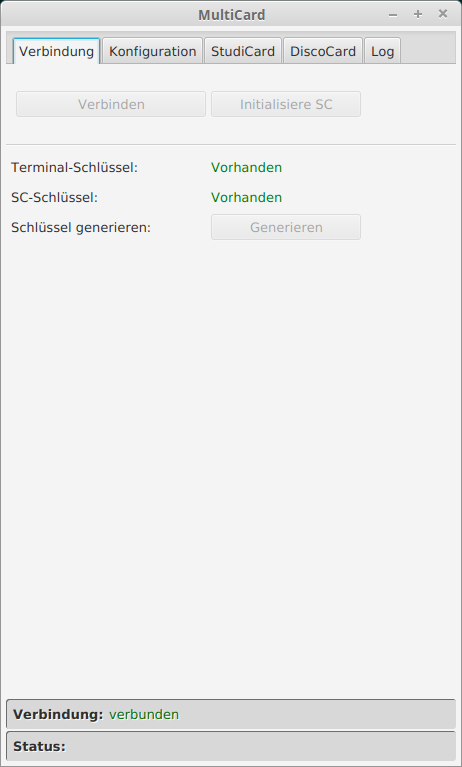
\includegraphics[scale=0.4]{Images/ConnectionTab}
\end{center}


\subsubsection{Configuration}
Dieser Tab ist im Wesentlichen dafür zuständig die Karte zu konfigurieren.
Zu diesen Konfigurationen gehören das Setzen von Studentennamen, Matrikelnummer, Raumfreischaltungen sowie Startwerte für Bonuspunkte und Geld.
Bei Klick auf diesen Tab werden alle aktuell gesetzten Informationen aus der Karte ausgelesen, welche für diese Anwendung relevant sind.

\begin{center}
	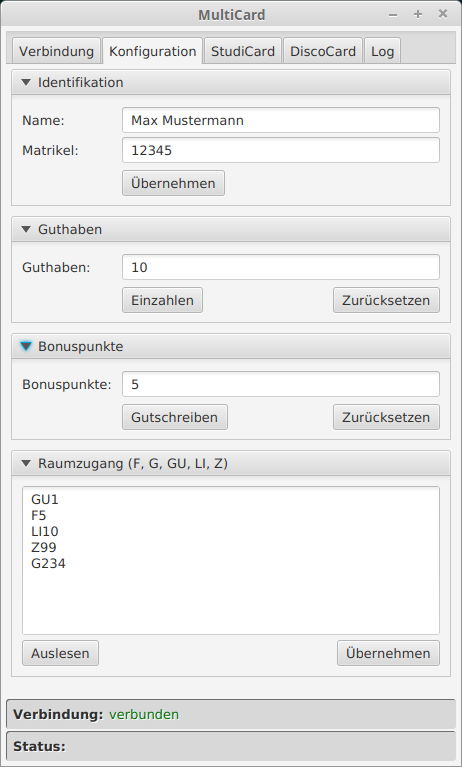
\includegraphics[scale=0.4]{Images/ConfigurationTab}
\end{center}


\subsubsection{Student}
In dem Student-Tab können zum Einen Studenteninformationen wie Name, Matrikelnummer und freigeschalteten Räumen ausgelesen werden.
Zum Anderen ist es möglich Geld auf seine SmartCard einzuzahlen sowie Geld auszugeben.
Üblicherweise wird Geld ausgegeben in dem man in der Mensa etwas isst.
Das Essen wird mit einfachem Geld bezahlen realisiert.
Bei Klick auf diesen Tab werden alle aktuell gesetzten Informationen aus der Karte ausgelesen, welche für diese Anwendung relevant sind.

\begin{center}
	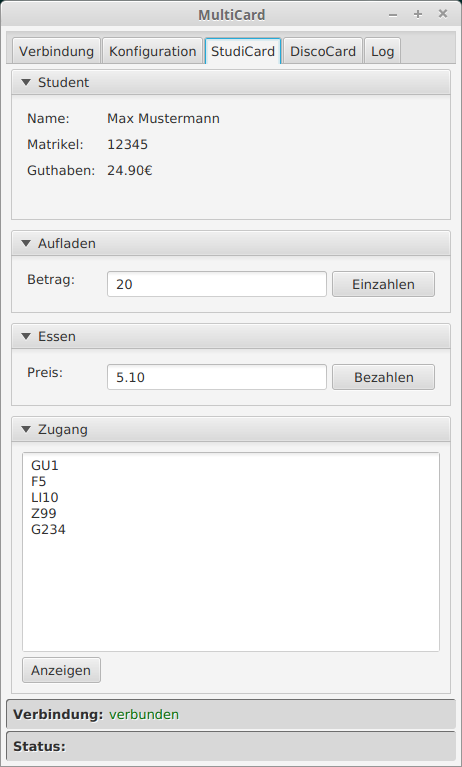
\includegraphics[scale=0.4]{Images/StudiCardTab}
\end{center}


\subsubsection{Disco}
Der Disco-Tab soll im Wesentlichen eine Beispielanwendung einer SmartCard in einer Disco demonstrieren.
Folgende Anwendung ist dabei realisiert:
Zunächst wird bei Betreten der Disco eine Eintrittsgebühr verlangt.
Diese Gebühr in Höhe von 10\texteuro{} muss bezahlt werden.
Die Gebühr kann mit Hilfe von Euro oder von Bonuspunkten von der Karte bezahlt werden.
Sollten nicht genügend Geld oder Bonuspunkte auf der Karte sein, so muss vorher das Guthaben auf der Karte erhöht werden.
Wenn man erfolgreich die Disco betreten hat, erhält man 10 Bonuspunkte.
In der Lokalität wird immer, wenn man etwas konsumiert, die Karte vorgezeigt und ein Getränk der Getränkeliste in der Karte hinzugefügt.
Ein Drittel des Euro-Wertes des Getränkes werden jeweils als Bonuspunkt verrechnet.

\begin{center}
	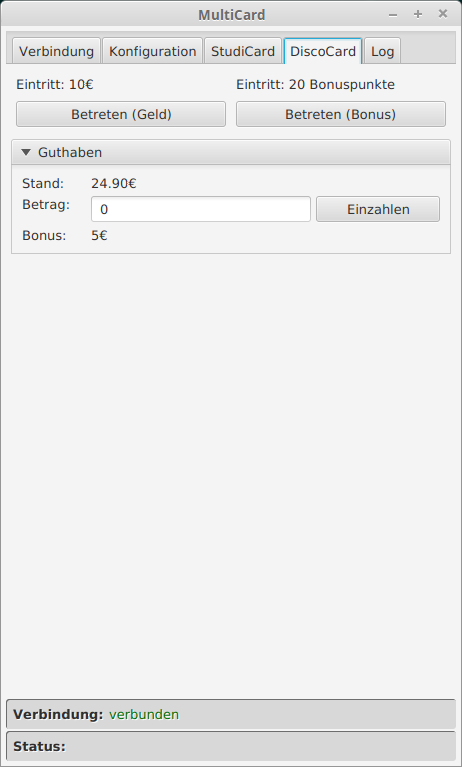
\includegraphics[scale=0.4]{Images/DiscoCardTabEntry}
\end{center}


Wenn der SmartCard-Nutzer nun die Disco verlässt, muss die SmartCard wieder vorgezeigt werden.
In diesem Vorgang werden alle konsumierten Getränke mit Hilfe von Guthaben und Bonuspunkten bezahlt.
Sollte nicht genug Guthaben vorhanden sein, so muss nach gezahlt werden, in dem das Guthaben der Karte erhöht wird.
Bereits bezahlte Getränke werden dabei jeweils auf der Karte aktualisiert.
Sind alle Getränke bezahlt, kann die Disco verlassen werden.
Sollte für das nach zahlen kein Geld vorhanden sein, so wäre es denkbar die Karte einzubehalten.
Durch die Zahlung des noch ausstehendes Geldes inklusive einer Mahngebühr, wird die Karte wieder ausgegeben.

\begin{center}
	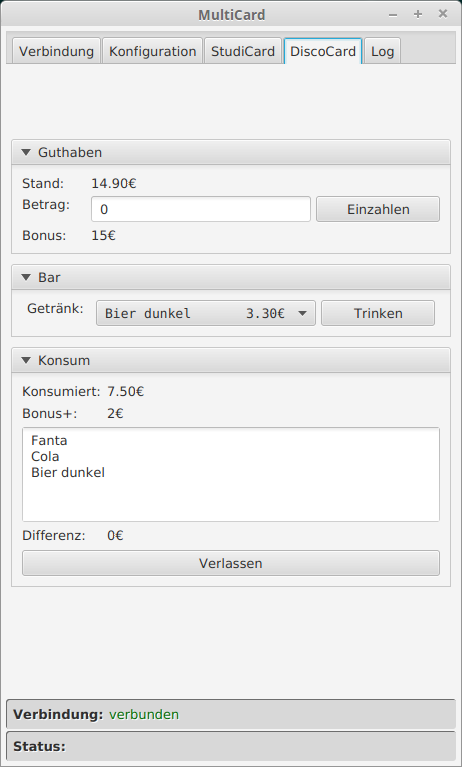
\includegraphics[scale=0.4]{Images/DiscoCardTabEntered}
\end{center}
 
\subsubsection{Logger und Statusinformationen}
Dieser Tab existiert im Wesentlichen um Informationen über die Kommunikation von OffCard- und OnCard-Anwendung darzustellen.
Das Logging in der Anwendung erleichterte die Entwicklung des Projektes, da so das finden von Fehlern etwas vereinfacht wurde.
In einer möglichen Release-Version der Anwendung könnte der Log-Tab ausgeblendet werden.

Zusätzlich zum Log-Tab existiert eine Status-Leiste, welche bei Ausführung von Befehlen stets Feedback gibt ob der Befehl korrekt ausgeführt wurde oder nicht.
Sollte ein Fehler auftreten, so wird an dieser Stelle der Fehler angezeigt.
Nach ein paar Sekunden wird die Statusleiste geleert.

\begin{center}
	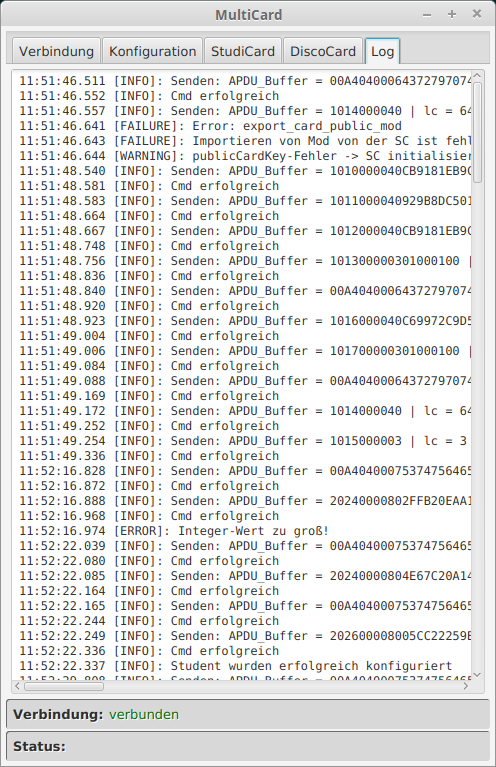
\includegraphics[scale=0.4]{Images/LogTab}
\end{center} 
 
\section{Fazit}
Im Verlauf des Projektes wurden alle Anforderungen des Projektes \qq{MultiCard} realisiert, sodass eine beispielhafte Implementierung einer SmartCard entstand.
Es wurden dabei OnCard- und OffCard-Teil eines solchen Projektes implementiert.

Die Realisierung des Projektes war dahingehend interessant, da ein anderer Anwendungszweck von Java aufgezeigt wurde.
Dabei ist die Programmiersprache kein reines Java sondern eine stark abgespeckte Variante.
Diese Variante erschwert das objektorientierte Programmieren.

Weiterhin kommt erschwerend hinzu, dass die Thematik \qq{JavaCard} anscheinend veraltet beziehungsweise zumindest nicht mehr für die breite Öffentlichkeit zugänglich ist.

Eine Realisierung von SmartCard mit Java besitzt außerdem den Nachteil das Java im Vergleich zu C beziehungsweise C++ speicherintensiver ist.
Es wäre denkbar SmartCard-Anwendungen mit Hilfe von C beziehungsweise C++ zu realisieren.

Alles in Allem entstand eine Anwendung, welche fast alle Funktionalitäten einer JavaCard aufzeigen.
Als Beispiel dafür seien genannt: Verschlüsselung, Applet-Firewall, Sharable Objects, \dots



\end{document}